% The preamble has been dumped out as out/presentationpreamble.fmt file. You can recreate that file by
% xelatex -ini -jobname="pinholepreamble" -output-directory=out "&xelatex pinholepreamble.tex\dump"
% 
% To compile you need to load that binary file using -fmt option
% xelatex -fmt out/pinholepreamble.fmt -output-directory=out pinhole.tex
%\documentclass[10pt, compress]{beamer}
\usetheme{m}
 
 \usepackage{booktabs} % for better tables
 \usepackage{media9} % for includemedia i.e. videos
 \usepackage{xcolor} % for more colors
 \usepackage{hyperref} % for links
 \usepackage{cutwin} % text wrapped around figures
 \usepackage[backend=bibtex]{biblatex} % fancy citations
 \usepackage{ifthen}
 
\usepackage{tikz}
\usetikzlibrary{shadows,trees}
\usetikzlibrary{shapes,calc,backgrounds}
\usetikzlibrary{intersections}
\usepgfplotslibrary{dateplot}


%\tikzset{external/system call={xelatex -fmt out/pinholepreamble.fmt \tikzexternalcheckshellescape -shell-escape -halt-on-error -interaction=batchmode -jobname "\image" "\texsource"}}
%

% transparency
%\setbeamercovered{transparent=15}

\title{Pinhole camera}
\date{\today}
\author{Vikas Dhiman\\ David Johnson\\ Jason J Corso}
\institute{University of Michigan}

\begin{document}
\maketitle
\begin{frame}{Pinhole camera}
  
\includegraphics{media/girl_looks.png}
\end{frame}

\section{Making a pinhole camera}
\begin{frame}{Step 1}
  \begin{columns}
    \begin{column}{0.4\textwidth}
      Take the plastic lid off the Pringles® can and wipe out the inside. (Save the lid!)
    \end{column}
    \begin{column}{0.6\textwidth}
      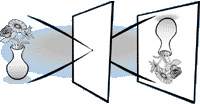
\includegraphics{media/upside_down_vase.png}
    \end{column}
  \end{columns}
\end{frame}

\begin{frame}{Step 2}
  \begin{columns}
    \begin{column}{0.4\textwidth}
Draw a line with the marker all the way around the can, about 2 inches up from the bottom. Have a grown-up cut along that line so the tube is in two pieces.
    \end{column}
    \begin{column}{0.6\textwidth}
      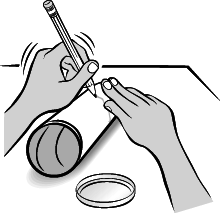
\includegraphics{media/hand_pencil.png}
    \end{column}
  \end{columns}
\end{frame}

\begin{frame}{Step 3}
  \begin{columns}
    \begin{column}{0.6\textwidth}
      \begin{itemize}
        \item 
          The shorter bottom piece has a metal end. With the thumbtack, make a hole in the center of the metal.
        \item
          We're going to use the plastic lid as a screen. If your lid is clear, you may need to apply a piece of wax paper, white tissue paper, or vellum to the lid to act as a translucent screen. Put the plastic lid onto the shorter piece. Put the longer piece back on top. Tape all the pieces together.
      \end{itemize}
    \end{column}
    \begin{column}{0.4\textwidth}
      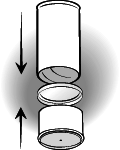
\includegraphics{media/can_cut_off.png}
    \end{column}
  \end{columns}
\end{frame}

\begin{frame}{Step 4}
  \begin{columns}
    \begin{column}{0.6\textwidth}
To keep light out of the tube, use a piece of aluminum foil that's about 1 foot long. Tape one end of the foil to the tube. Wrap the foil all the way around the tube twice, then tape the loose edge of the foil closed. If you have extra foil at the top, just tuck it neatly inside the tube.
    \end{column}
    \begin{column}{0.4\textwidth}
      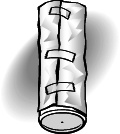
\includegraphics{media/can_cover.png}
    \end{column}
  \end{columns}
\end{frame}

\begin{frame}{Pinhole camera is ready to use}
  
\includegraphics{media/girl_looks.png}
\end{frame}

\section{How does it works}
\begin{frame}{}
  
\end{frame}

\end{document}
